\subsection{Citus: Distributed PostgreSQL}

Citus merupakan \textit{distributed database engine} untuk PostgreSQL yang menangani kebutuhan skalabilitas pada ekosistem PostgreSQL \parencite{citus}. Sebagai sebuah \textit{extension}, Citus menjaga \textit{compatibility} dengan PostgreSQL, sehingga dapat digunakan dengan PostgreSQL versi terbaru.

Sebuah \textit{cluster} memiliki banyak \textit{nodes} yang terspesialisasi menjadi \textit{coordinator} dan \textit{worker}. Aplikasi mengirimkan \textit{query} kepada \textit{coordinator} dan diteruskan kepada \textit{worker} terkait atau menggabungkan hasil. Pendekatan ini memungkinkan setiap \textit{node} mampu memproses \textit{write} request sehingga pemrosesan bisa dilakukan secara parallel.

Selain itu, berikut adalah fitur lain \textit{extension} Citus:

\begin{enumerate}
    \item \textit{Distributed tables} dibagi ke seluruh kluster node untuk menggabungkan \textit{machine resources}.
    \item \textit{Referenced tables} direplikasi ke seluruh node untuk kebutuhan \textit{join} dan \textit{foreign key}, sehingga kinerja \textit{read} semakin baik.
    \item \textit{Distributed query engine routes} dan memparallelkan operasi pada tabel terdistribusi ke seluruh kluster.
\end{enumerate}

Citus memiliki dua model \textit{sharding}, yaitu \textit{row-based sharding} dan \textit{schema based sharding}.

\begin{figure}[ht]
    \centering
    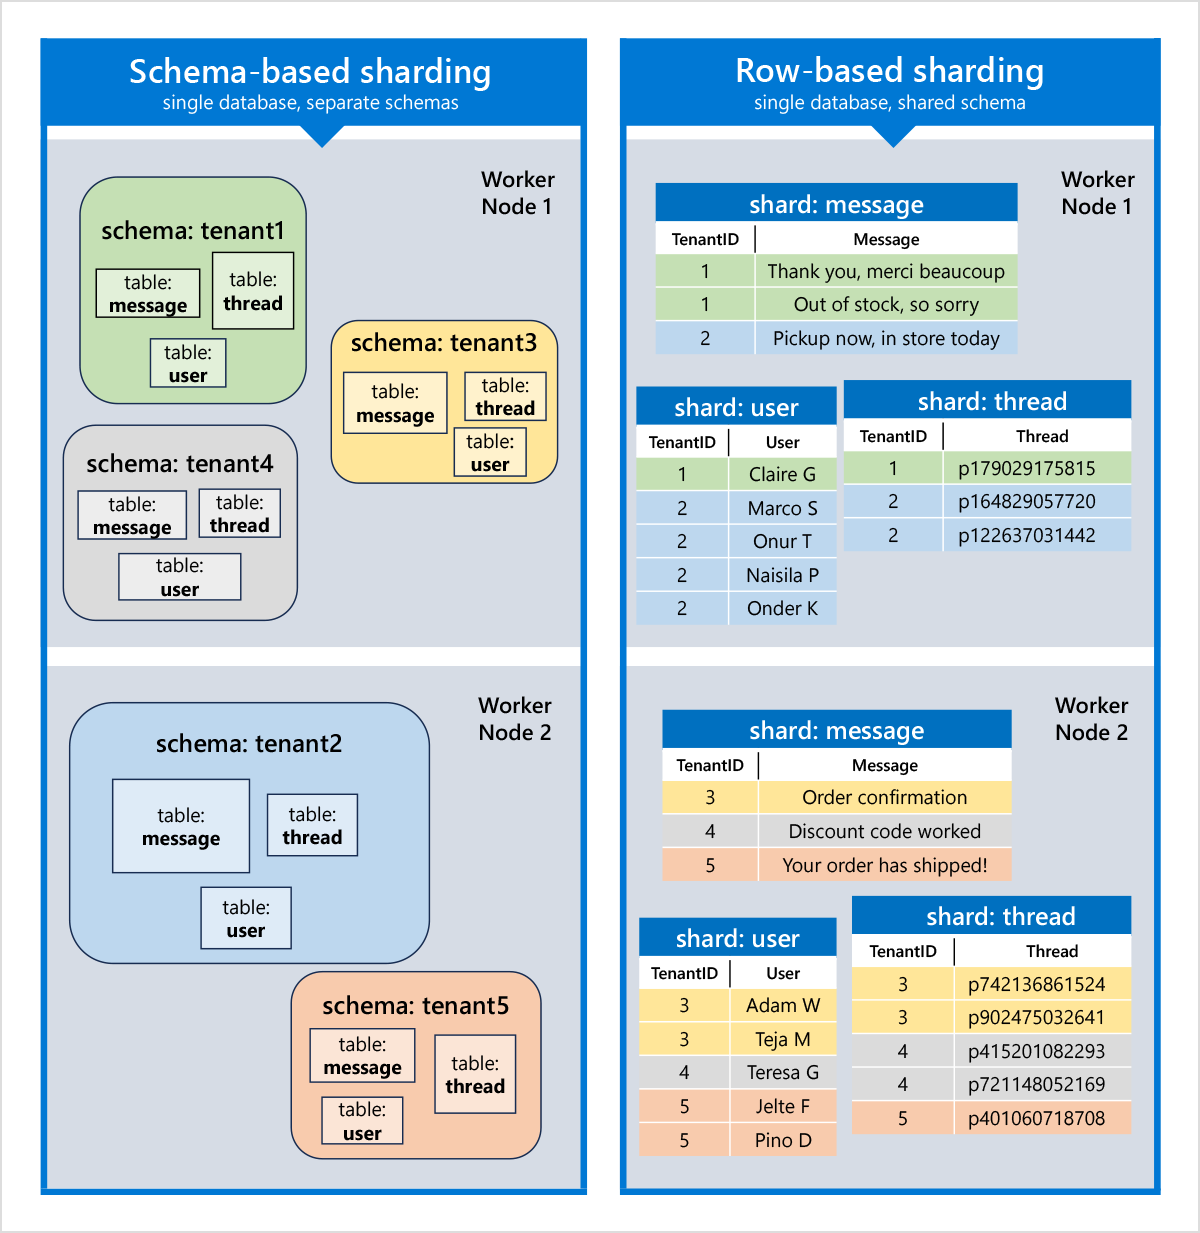
\includegraphics[width=0.8\textwidth]{resources/chapter-2/row-vs-schema-sharding.png}
    \caption{\textit{Schema-based sharding vs row-based sharding \parencite{schemaBasedSharding}}}
    \label{fig:row-vs-schema-sharding}
\end{figure}

